\documentclass[10pt,journal,compsoc,onecolumn]{IEEEtran}
\usepackage[utf8]{inputenc}
\usepackage{amsmath,amsfonts,amssymb}
\usepackage{amsthm}
\usepackage{graphicx}
\usepackage{cite}
\usepackage{textcomp}
\usepackage{tikz}
\usetikzlibrary{arrows,positioning,shapes.geometric}
\usepackage{booktabs}
\usepackage{url}
\usepackage{listings}
\usepackage{xcolor}
\usetikzlibrary{arrows,arrows.meta,positioning,shapes.geometric,calc,fit}

\definecolor{codegreen}{rgb}{0,0.5,0}
\definecolor{codegray}{rgb}{0.4,0.4,0.4}
\definecolor{codepurple}{rgb}{0.5,0,0.7}
\definecolor{backcolour}{rgb}{0.97,0.97,0.97}
\definecolor{keywordblue}{rgb}{0.0,0.2,0.7}

\lstdefinestyle{sqlstyle}{
    backgroundcolor=\color{backcolour},   
    commentstyle=\color{codegreen}\itshape,
    keywordstyle=\color{keywordblue}\bfseries,
    numberstyle=\tiny\color{codegray},
    stringstyle=\color{codepurple},
    basicstyle=\ttfamily\footnotesize,
    breakatwhitespace=false,         
    breaklines=true,                 
    captionpos=b,                    
    keepspaces=true,                 
    numbers=left,                    
    numbersep=5pt,                  
    showspaces=false,                
    showstringspaces=false,
    showtabs=false,                  
    tabsize=2,
    frame=single,
    rulecolor=\color{black!20}
}
\lstset{style=sqlstyle}

\newtheorem{theorem}{Theorem}
\newtheorem{lemma}[theorem]{Lemma}
\newtheorem{definition}[theorem]{Definition}
\newtheorem{corollary}[theorem]{Corollary}

\begin{document}

\title{Architectural Foundations of Relational Database Integrity: Key Taxonomy, Physical Storage Indexing, Referential Constraints, and Mutation Mechanics in SQL Systems}

\IEEEtitleabstractindextext{%
\begin{abstract}
In relational database management systems (RDBMS), structural integrity and storage efficiency depend fundamentally on key constraints and referential enforcement protocols. While classical database literature often obscures implementation realities behind abstract relational mathematics, production engineering requires a concrete understanding of physical storage layout, B+ Tree index clustering, memory-cache locality, and foreign key state transitions. This paper presents an exhaustive architectural analysis of relational keys, constraint enforcement, and SQL CRUD operations based on modern database engines such as MySQL InnoDB. We examine the taxonomy of database keys---distinguishing candidate keys, surrogate primary keys, natural composite keys, and foreign keys. We analyze the physical mechanics of primary key selection, demonstrating how data types, byte footprints, lexicographic versus integer sorting, and immutability directly govern B+ Tree page fan-out and I/O efficiency. Furthermore, we dissect foreign key constraints and referential integrity, tracing the exact consequences of parent record mutations. We formalize the operational mechanics of ON UPDATE and ON DELETE actions---CASCADE, SET NULL, and RESTRICT/NO ACTION---contrasting high-impact architectural patterns across enterprise domains, from unified single sign-on user lifecycles (Google Account cascade deletion) to regulatory audit trail preservation (Amazon order history decoupling). Finally, we demonstrate the operational lifecycle of database schemas through production-grade SQL DDL and DML workflows, providing concrete patterns for resilient schema design in high-throughput transactional systems.
\end{abstract}

\begin{IEEEkeywords}
Relational Databases, SQL CRUD Mechanics, Candidate Keys, Primary Keys, Composite Keys, Foreign Keys, Referential Integrity, ON UPDATE CASCADE, ON DELETE SET NULL, Clustered Index, B+ Tree, InnoDB Storage Engine, Sakila Database
\end{IEEEkeywords}
}

\maketitle
\IEEEdisplaynontitleabstractindextext
\IEEEpeerreviewmaketitle

\section{Introduction and Relational Architecture Foundations}
\label{sec:intro}

Modern software engineering systems depend fundamentally on Relational Database Management Systems (RDBMS) to guarantee data persistence, transaction safety, and architectural consistency. While contemporary industry discourse frequently highlights distributed NoSQL key-value stores and document databases, relational systems such as MySQL (InnoDB), PostgreSQL, and Oracle remain the core transactional backbone for financial settlement platforms, enterprise identity providers, and mission-critical business workflows.

At the heart of the relational architecture lies a strict separation between logical schema definitions and physical storage mechanics. Logically, data is structured as two-dimensional relations (tables) consisting of defined attributes (columns) and tuples (rows). Physically, database engines organize these records across storage blocks, memory buffers, and tree-structured indexes. 

The primary mechanism that bridges logical intent with physical correctness is the relational constraint framework. Without constraints, databases degrade into disorganized data heaps plagued by orphan records, dangling pointers, inconsistent update anomalies, and corrupt business states. Relational constraints---predominantly Candidate Keys, Primary Keys, Unique Constraints, and Foreign Key relationships---provide hard, system-level guarantees that the database engine enforces on every single transactional mutation.

This research paper provides an exhaustive, practice-oriented engineering examination of relational database integrity, key taxonomy, physical storage indexing, and mutation mechanics. Derived from production database analysis and foundational architectural principles, this paper explicitly eliminates abstract mathematical formalism in favor of practical systems engineering, physical memory and disk layout mechanics, concrete Structured Query Language (SQL) Data Definition Language (DDL) and Data Manipulation Language (DML) workflows, and real-world enterprise case studies.

% -----------------------------------------------------------------------------
\section{Taxonomy and Structural Roles of Relational Keys}
\label{sec:key_taxonomy}

In a relational database, a key is an attribute or combination of attributes that serves to uniquely identify, order, or interlink tuples across relations. Understanding the precise architectural boundaries between different key classifications is essential for robust database modeling.

\subsection{Candidate Keys}
A Candidate Key is any minimal set of attributes within a relation that possesses the uniqueness property: no two distinct tuples in the relation can have identical values across these attributes. A relation may possess multiple candidate keys simultaneously.

For instance, consider a modern university or academy student entity containing the following attributes:
\begin{itemize}
    \item \texttt{id}: A system-generated auto-incrementing integer.
    \item \texttt{email}: The official institutional email address (e.g., \texttt{student@academy.edu}).
    \item \texttt{phone\_number}: A unique mobile contact number.
    \item \texttt{national\_id} (e.g., Aadhar, Social Security Number): A government-issued civilian identification number.
\end{itemize}

Each of these four individual attributes qualifies as a Candidate Key because each one independently guarantees tuple uniqueness. If an engineer searches the relation using any of these columns, at most one single student tuple will be returned.

\subsection{The Primary Key: The Chosen Relation Anchor}
While a table may have several Candidate Keys, a relational table can possess exactly one Primary Key. The Primary Key is the single Candidate Key formally designated by the database designer to serve as the physical identity anchor for that relation. 

The Primary Key imposes two fundamental system constraints:
\begin{enumerate}
    \item \textbf{Entity Uniqueness}: No duplicate values are permitted under any circumstance.
    \item \textbf{Non-Nullability}: The primary key column cannot contain null values. Every tuple must possess a known, concrete identifier.
\end{enumerate}

The choice of which Candidate Key should be promoted to the Primary Key is not arbitrary; it directly governs the physical storage layout, index depth, and query throughput of the database engine, as analyzed in Section~\ref{sec:pk_engineering}.

\subsection{Composite Primary Keys}
When no single attribute provides unique identification, or when modeling many-to-many junction tables, a Composite Key is utilized. A Composite Key is a primary key composed of two or more columns whose combined values are guaranteed to be unique across the relation.

A canonical example is an enrollment mapping table connecting students with courses:
\begin{itemize}
    \item \texttt{student\_id}: Foreign key pointing to the student relation.
    \item \texttt{course\_id}: Foreign key pointing to the course relation.
    \item \texttt{enrollment\_date}: Timestamp of registration.
\end{itemize}
In this schema, neither \texttt{student\_id} nor \texttt{course\_id} is individually unique, because a single student can enroll in multiple courses, and a single course contains multiple students. However, the compound pair \texttt{(student\_id, course\_id)} is unique, preventing duplicate registrations for the same course.

\subsection{Alternate and Secondary Keys}
All Candidate Keys that are not selected as the Primary Key are classified as Alternate Keys. In production SQL implementations, Alternate Keys are enforced through \texttt{UNIQUE} constraints accompanied by secondary indexes. Unlike primary keys, standard SQL permits alternate key columns to contain \texttt{NULL} values unless an explicit \texttt{NOT NULL} constraint is applied.

\subsection{Foreign Keys: Cross-Table Referential Links}
A Foreign Key is an attribute or collection of attributes in a child table that refers directly to the Primary Key (or a unique key) of a parent table. The Foreign Key establishes an enforceable parent-child bond, ensuring that a record in the child table cannot point to a non-existent entity in the parent table.

\begin{table*}[t]
\caption{Comprehensive Comparison of Relational Key Classifications}
\label{tab:key_taxonomy}
\centering
\begin{tabular}{p{2.8cm}p{2.2cm}p{2.8cm}p{3.8cm}p{4.0cm}}
\toprule
\textbf{Key Type} & \textbf{Multiplicity} & \textbf{Nullability} & \textbf{Core Purpose} & \textbf{Production Example} \\
\midrule
\textbf{Candidate Key} & Multiple permitted per table & Permitted unless constrained & Defines any minimal unique attribute set capable of row identification & \texttt{email}, \texttt{phone\_number}, \texttt{national\_id} \\
\midrule
\textbf{Primary Key (PK)} & Exactly one per table & Strictly disallowed (\texttt{NOT NULL}) & Physical clustered index anchor, primary entity identifier & \texttt{id INT AUTO\_INCREMENT PRIMARY KEY} \\
\midrule
\textbf{Composite Key} & One composite PK per table & Strictly disallowed on key columns & Ensures uniqueness across multi-attribute combinations (junction tables) & \texttt{PRIMARY KEY (student\_id, batch\_id)} \\
\midrule
\textbf{Alternate Key} & Multiple permitted per table & Allowed (unless marked \texttt{NOT NULL}) & Secondary candidate keys requiring uniqueness enforcement & \texttt{email VARCHAR(255) UNIQUE} \\
\midrule
\textbf{Foreign Key (FK)} & Multiple permitted per table & Permitted if optional (NULL allowed) & Establishes referential integrity to a parent relation & \texttt{batch\_id INT REFERENCES batches(b\_id)} \\
\bottomrule
\end{tabular}
\end{table*}

% -----------------------------------------------------------------------------
\section{Physical Storage Mechanics and Primary Key Engineering}
\label{sec:pk_engineering}

A frequent misconception in software engineering is treating primary key selection as a purely logical exercise. In high-performance relational engines like MySQL (InnoDB), the primary key directly dictates the physical organization of data on disk through Clustered Indexing.

\subsection{The Clustered Index and B+ Tree Organization}
In MySQL InnoDB, table data is not stored as an unordered flat file. Instead, the entire physical table is a B+ Tree structured index, termed the Clustered Index. The leaf pages of the Clustered Index do not contain pointers to data; they contain the actual row payload (all column values for that tuple).

The governing rules of InnoDB clustered indexing are:
\begin{enumerate}
    \item The physical arrangement of rows on disk precisely mirrors the ascending sorted order of the Primary Key.
    \item By default, MySQL orders result sets based on the primary key index unless an explicit \texttt{ORDER BY} clause overrides it.
    \item Secondary indexes (non-primary indexes) do not store physical disk offsets; instead, each secondary index leaf node stores the Primary Key value of the corresponding row. Consequently, any query utilizing a secondary index performs a two-stage lookup: first searching the secondary index B+ Tree to find the Primary Key, and then traversing the Primary Key Clustered B+ Tree to retrieve the full row payload.
\end{enumerate}

\begin{figure*}[htbp]
\centering
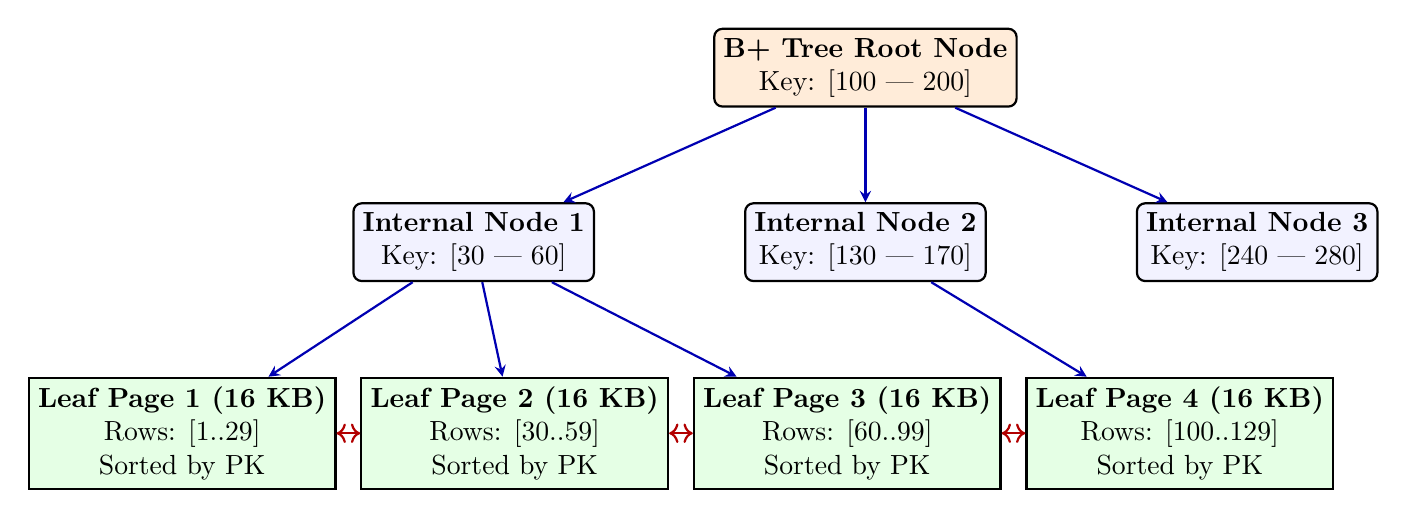
\begin{tikzpicture}[
    node distance=1.2cm and 1.0cm,
    box/.style={draw, rectangle, rounded corners=3pt, thick, align=center, fill=blue!5, minimum width=2.8cm, minimum height=0.9cm},
    leaf/.style={draw, rectangle, thick, align=center, fill=green!10, minimum width=3.2cm, minimum height=1.1cm},
    arrow/.style={->, >=stealth, thick, color=blue!70!black}
]
    % Root Node
    \node[box, fill=orange!15] (root) {\textbf{B+ Tree Root Node}\\Key: [100 | 200]};
    
    % Internal Level Nodes
    \node[box, below left=1.2cm and 1.5cm of root] (int1) {\textbf{Internal Node 1}\\Key: [30 | 60]};
    \node[box, below=1.2cm of root] (int2) {\textbf{Internal Node 2}\\Key: [130 | 170]};
    \node[box, below right=1.2cm and 1.5cm of root] (int3) {\textbf{Internal Node 3}\\Key: [240 | 280]};
    
    % Leaf Level Nodes
    \node[leaf, below left=1.2cm and 0.2cm of int1] (leaf1) {\textbf{Leaf Page 1 (16 KB)}\\Rows: [1..29]\\Sorted by PK};
    \node[leaf, right=0.3cm of leaf1] (leaf2) {\textbf{Leaf Page 2 (16 KB)}\\Rows: [30..59]\\Sorted by PK};
    \node[leaf, right=0.3cm of leaf2] (leaf3) {\textbf{Leaf Page 3 (16 KB)}\\Rows: [60..99]\\Sorted by PK};
    \node[leaf, right=0.3cm of leaf3] (leaf4) {\textbf{Leaf Page 4 (16 KB)}\\Rows: [100..129]\\Sorted by PK};
    
    % Arrows
    \draw[arrow] (root) -- (int1);
    \draw[arrow] (root) -- (int2);
    \draw[arrow] (root) -- (int3);
    
    \draw[arrow] (int1) -- (leaf1);
    \draw[arrow] (int1) -- (leaf2);
    \draw[arrow] (int1) -- (leaf3);
    \draw[arrow] (int2) -- (leaf4);
    
    % Leaf Doubly Linked List
    \draw[<->, thick, color=red!70!black] (leaf1) -- (leaf2);
    \draw[<->, thick, color=red!70!black] (leaf2) -- (leaf3);
    \draw[<->, thick, color=red!70!black] (leaf3) -- (leaf4);
\end{tikzpicture}
\caption{Architectural layout of an InnoDB Clustered Index B+ Tree. The table rows reside directly within leaf pages ordered strictly by Primary Key. Leaf pages are doubly linked for sequential range scans.}
\label{fig:clustered_index}
\end{figure*}

\subsection{Engineering Criteria for Optimal Primary Key Selection}
Because the Primary Key forms the physical backbone of the database, choosing the correct attribute requires balancing four core engineering metrics:

\subsubsection{1. Storage Footprint and Page Fan-Out}
InnoDB manages storage in fixed-size pages of 16 Kilobytes (16,384 bytes). The number of index entries that can fit inside an internal B+ Tree page is known as the index fan-out. 
\begin{itemize}
    \item A standard 4-byte signed integer (\texttt{INT}) provides over 2.14 billion unique values. An 8-byte integer (\texttt{BIGINT}) provides over 9 quintillion values.
    \item A 12-digit string or 64-byte national identity string (such as an Aadhar number or UUID representation) consumes 16 to 64 bytes per entry.
\end{itemize}
When a primary key consumes 64 bytes compared to 4 bytes, the page fan-out drops dramatically. An internal page that could have held thousands of 4-byte key pointers can now hold only a fraction of that number. As fan-out decreases:
\begin{itemize}
    \item The total tree height increases, requiring additional disk page reads for every point lookup.
    \item Every secondary index in the table balloons in size, because every secondary index record must embed a copy of the primary key.
    \item The database buffer pool in system memory becomes saturated with large index pages, forcing cache evictions and degrading overall system throughput.
\end{itemize}

\subsubsection{2. Sorting and Comparison Performance}
In B+ Tree operations (searches, node splits, binary searches within pages), key comparisons occur millions of times per second. 
\begin{itemize}
    \item \textbf{Numeric Keys}: Integer comparisons are executed in a single CPU cycle via hardware register instructions.
    \item \textbf{String Keys}: Lexicographical string comparisons require multi-byte memory traversals, collation rule evaluations, and variable-length decoding, resulting in significantly higher CPU overhead.
\end{itemize}
Consequently, sorting on numeric primary keys is orders of magnitude faster than sorting on textual keys.

\subsubsection{3. Strict Immutability}
A good Primary Key must \textbf{never change}. 
If a primary key value is modified via an \texttt{UPDATE} statement:
\begin{enumerate}
    \item The database engine cannot simply modify the value in-place. Because rows are physically ordered by primary key, changing the key forces the engine to delete the row from its current physical page and insert it into a completely different page.
    \item This row relocation frequently triggers costly B+ Tree page splits and rebalancing operations.
    \item Every secondary index in the table must be updated to replace the old primary key pointer with the new primary key value.
    \item If foreign keys in child tables reference this primary key, cascading update locks must ripple through the entire relational dependency graph, holding table and row locks that stall concurrent transactions.
\end{enumerate}

\subsubsection{4. Surrogate Keys vs. Natural Keys}
A Natural Key is an attribute that exists organically in the real world (e.g., email address, phone number, national identity number). A Surrogate Key is a synthetic, system-generated identifier with no business meaning (e.g., an auto-incrementing integer or sequential snowflake identifier).

Real-world attributes make exceptionally poor primary keys:
\begin{itemize}
    \item \textbf{Phone numbers} change when users switch cellular carriers or travel internationally.
    \item \textbf{Email addresses} change due to rebranding, personal preference, or typos during user registration.
    \item \textbf{National IDs (Aadhar / SSN)} carry severe regulatory, data privacy, and encryption compliance requirements (e.g., GDPR, HIPAA, PCI-DSS). Storing national identification strings across every secondary index and foreign key column creates severe compliance hazards.
\end{itemize}
Therefore, production systems universally adopt surrogate integer keys as Primary Keys, while enforcing natural key uniqueness through alternate unique constraints.

\begin{table}[htbp]
\caption{Primary Key Selection Evaluation Matrix}
\label{tab:pk_evaluation}
\centering
\begin{tabular}{p{2.5cm}p{1.5cm}p{2.2cm}p{2.2cm}p{4.2cm}}
\toprule
\textbf{Attribute} & \textbf{Size} & \textbf{Sort Speed} & \textbf{Immutability} & \textbf{Engineering Verdict} \\
\midrule
\texttt{id (INT / BIGINT)} & 4 / 8 Bytes & Single-cycle numeric & 100\% Static & \textbf{Optimal}: Maximum fan-out, compact secondary indexes. \\
\midrule
\texttt{phone\_number} & 10--15 Bytes & Moderate & Low (User changes) & \textbf{Poor}: Subject to mutation and formatting shifts. \\
\midrule
\texttt{email} & 30--64 Bytes & Slow (Lexicographic) & Low (User updates) & \textbf{Unsuitable}: High storage overhead, inflates all secondary indexes. \\
\midrule
\texttt{national\_id} (Aadhar) & 12--64 Bytes & Slow (String checks) & Moderate & \textbf{Hazardous}: Privacy risks, regulatory compliance overhead. \\
\bottomrule
\end{tabular}
\end{table}

% -----------------------------------------------------------------------------
\section{Foreign Keys and Referential Integrity Foundations}
\label{sec:referential_integrity}

The fundamental power of the relational model is its ability to establish relationships between independent entities without data duplication. This is achieved through Foreign Keys.

\subsection{The Parent-Child Relational Bond}
When two tables are related, they assume a hierarchical Parent-Child dynamic:
\begin{itemize}
    \item \textbf{Parent Table}: The relation holding the authoritative entity and master key (typically its primary key).
    \item \textbf{Child Table}: The relation containing the referencing foreign key attribute pointing back to the parent.
\end{itemize}

Consider an educational academy system comprising \texttt{batches} and \texttt{students}:
\begin{itemize}
    \item \texttt{batches} is the \textbf{Parent Table}, containing batch identifier \texttt{b\_id} (Primary Key), \texttt{batch\_name}, and \texttt{instructor\_name}.
    \item \texttt{students} is the \textbf{Child Table}, containing student identifier \texttt{s\_id} (Primary Key), \texttt{student\_name}, \texttt{psp} (Problem Solving Percentage), and \texttt{batch\_id} (Foreign Key referencing \texttt{batches.b\_id}).
\end{itemize}

\begin{figure}[htbp]
\centering
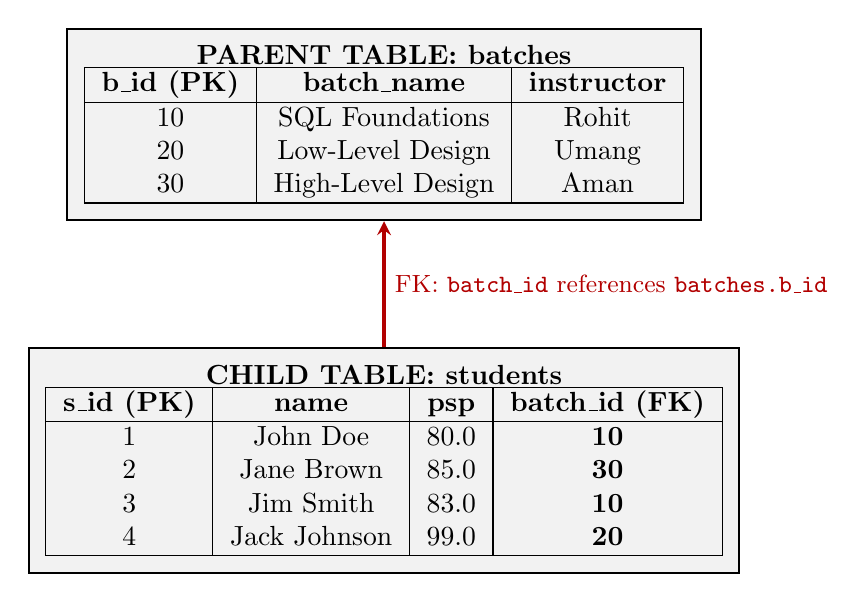
\begin{tikzpicture}[
    table/.style={draw, rectangle, thick, align=center, fill=gray!10, minimum width=6.5cm, inner sep=6pt},
    fkarrow/.style={->, >=stealth, very thick, color=red!70!black}
]
    % Parent Table
    \node[table] (parent) {
        \textbf{PARENT TABLE: batches}\\
        \begin{tabular}{|c|c|c|}
            \hline
            \textbf{b\_id (PK)} & \textbf{batch\_name} & \textbf{instructor} \\
            \hline
            10 & SQL Foundations & Rohit \\
            20 & Low-Level Design & Umang \\
            30 & High-Level Design & Aman \\
            \hline
        \end{tabular}
    };
    
    % Child Table
    \node[table, below=1.6cm of parent] (child) {
        \textbf{CHILD TABLE: students}\\
        \begin{tabular}{|c|c|c|c|}
            \hline
            \textbf{s\_id (PK)} & \textbf{name} & \textbf{psp} & \textbf{batch\_id (FK)} \\
            \hline
            1 & John Doe & 80.0 & \textbf{10} \\
            2 & Jane Brown & 85.0 & \textbf{30} \\
            3 & Jim Smith & 83.0 & \textbf{10} \\
            4 & Jack Johnson & 99.0 & \textbf{20} \\
            \hline
        \end{tabular}
    };
    
    % Foreign Key Reference Arrow
    \draw[fkarrow] (child.north) -- node[midway, right, font=\small] {FK: \texttt{batch\_id} references \texttt{batches.b\_id}} (parent.south);
\end{tikzpicture}
\caption{The Parent-Child Foreign Key relationship between \texttt{batches} and \texttt{students}. The child table references the primary key of the parent table to guarantee referential validity.}
\label{fig:fk_relationship}
\end{figure}

\subsection{The Danger of Orphan Records and Dangling References}
What happens if the database engine does not enforce foreign key constraints?
Suppose an administrator executes:
\begin{verbatim}
DELETE FROM batches WHERE b_id = 20;
\end{verbatim}
If the relational bond is not enforced at the storage engine level:
\begin{enumerate}
    \item The batch record with \texttt{b\_id = 20} is deleted from disk.
    \item The student record for ``Jack Johnson'' (\texttt{s\_id = 4}) still holds \texttt{batch\_id = 20}.
    \item Student 4 has now become an \textbf{Orphan Record}. The value 20 in \texttt{batch\_id} is a \textbf{Dangling Pointer} referencing an entity that no longer exists in reality.
\end{enumerate}

Orphan records cause immediate downstream systemic failure:
\begin{itemize}
    \item \textbf{Application Crashes}: Application servers attempting to load batch details for Student 4 execute SQL inner joins that silently drop the student from reports, or trigger null pointer exceptions in backend microservices.
    \item \textbf{Data Inconsistency}: Automated billing engines continue charging students for batches that were decommissioned.
    \item \textbf{Corrupt Analytical Aggregations}: Analytical data pipelines fail to balance foreign key dimensions, halting business intelligence reporting.
\end{itemize}

\subsection{Engine-Level Referential Constraint Interception}
To eliminate orphan records, relational database engines enforce \textbf{Referential Integrity}. Referential integrity dictates that any foreign key value present in a child relation must match an existing primary key value in the parent relation, or be set explicitly to \texttt{NULL} (if nullability is permitted).

The RDBMS intercepts every data mutation before committing it to disk:
\begin{itemize}
    \item \textbf{Child Insertion Validation}: If an application attempts to insert a student with \texttt{batch\_id = 50}, but the \texttt{batches} table only contains identifiers 10, 20, and 30, the engine aborts the transaction immediately with a foreign key violation error (e.g., MySQL Error 1452: \textit{Cannot add or update a child row: a foreign key constraint fails}).
    \item \textbf{Parent Modification Interception}: If an application attempts to delete a parent batch or change its primary key while child student rows point to it, the engine enforces configured referential action rules.
\end{itemize}

\subsection{DDL Creation and Destruction Dependencies}
Referential constraints introduce a strict directional dependency in SQL Data Definition Language (DDL) execution:
\begin{enumerate}
    \item \textbf{Creation Order}: The Parent table \textbf{must} be created before the Child table. A table definition that declares a foreign key referencing a non-existent parent table will fail compilation immediately.
    \item \textbf{Destruction Order}: The Child table \textbf{must} be dropped before the Parent table can be deleted. Attempting to execute \texttt{DROP TABLE batches;} while \texttt{students} exists will result in MySQL Error 1217: \textit{Cannot delete or update a parent table: a foreign key constraint fails}.
\end{enumerate}

% -----------------------------------------------------------------------------
\section{Mutation Dynamics: Operational Semantics of ON UPDATE and ON DELETE}
\label{sec:mutation_rules}

When a record in a parent table undergoes mutation---specifically when a parent row is deleted or its primary key value is updated---the database engine must determine how to handle dependent child rows. SQL provides four standardized behavioral policies defined via the \texttt{ON UPDATE} and \texttt{ON DELETE} clauses.

\subsection{RESTRICT / NO ACTION (The Defensive Default)}
In standard MySQL InnoDB, if no explicit rule is specified, the engine applies \texttt{RESTRICT} (which behaves identically to \texttt{NO ACTION} in standard transaction contexts).

\begin{itemize}
    \item \textbf{Behavior}: If any child row references the parent record, the database engine prohibits any modification or deletion of that parent record. The transaction is instantly aborted and rolled back.
    \item \textbf{Operational Workflow}: To delete batch 20, an administrator must first manually reassign or delete all students belonging to batch 20. Only after zero child records reference batch 20 will the engine permit the deletion of batch 20.
    \item \textbf{Use Case}: Mission-critical financial ledgers and core entity master records where silent automatic modifications would introduce operational ambiguity.
\end{itemize}

\subsection{CASCADE (Propagative Synchronization)}
The \texttt{CASCADE} action instructs the database engine to automatically propagate parent mutations down to all dependent child records.

\begin{itemize}
    \item \textbf{ON UPDATE CASCADE}: If parent batch 10 has its identifier updated to 15 (\texttt{UPDATE batches SET b\_id = 15 WHERE b\_id = 10}), the database engine automatically updates the \texttt{batch\_id} column in all student rows referencing 10 to 15. Referential integrity is preserved automatically without human intervention.
    \item \textbf{ON DELETE CASCADE}: If parent batch 10 is deleted (\texttt{DELETE FROM batches WHERE b\_id = 10}), the engine automatically executes deletions for \textbf{every single student} enrolled in batch 10.
    \item \textbf{Production Risk}: While \texttt{ON UPDATE CASCADE} is generally safe and beneficial, \texttt{ON DELETE CASCADE} is hazardous. Deleting a parent category or batch could unintentionally wipe out thousands of dependent student records.
\end{itemize}

\subsection{SET NULL (Decoupled Disassociation)}
The \texttt{SET NULL} action breaks the relational bond upon parent modification without destroying the child record.

\begin{itemize}
    \item \textbf{Behavior}: When the referenced parent record is deleted or updated, the foreign key column in all dependent child rows is automatically set to \texttt{NULL}.
    \item \textbf{Prerequisite}: The foreign key column in the child table \textbf{must} be nullable (it cannot have the \texttt{NOT NULL} constraint).
    \item \textbf{Operational Meaning}: In our academy system, if batch 20 is deleted, student 4 (Jack Johnson) is not deleted from the database. Instead, Jack's \texttt{batch\_id} becomes \texttt{NULL}. Jack remains an active student in the academy system, classified as unassigned and ready to be enrolled into a future batch.
    \item \textbf{Use Case}: Optional relationships where the child entity has an independent existence outside the lifespan of the parent entity.
\end{itemize}

\subsection{SET DEFAULT}
Under \texttt{SET DEFAULT}, when a parent record is mutated, the child table foreign key column is automatically assigned a pre-configured default value (e.g., reassigning unbatched students to a designated Holding Batch with \texttt{b\_id = 1}). While supported in standard SQL and PostgreSQL, MySQL InnoDB does not support \texttt{SET DEFAULT} foreign key actions.

\begin{table*}[t]
\caption{Comparative Matrix of Referential Action Rules}
\label{tab:action_rules}
\centering
\begin{tabular}{p{2.5cm}p{3.2cm}p{3.5cm}p{3.0cm}p{3.0cm}}
\toprule
\textbf{Action Rule} & \textbf{Parent Deletion Behavior} & \textbf{Parent Key Update Behavior} & \textbf{Child Data Retention} & \textbf{Primary Risk Profile} \\
\midrule
\textbf{RESTRICT / NO ACTION} & Rejects deletion if child rows exist (Error 1451). & Rejects update if child rows exist (Error 1451). & 100\% preserved; blocks unsafe operations. & Application errors if deletions are not preceded by manual cleanup. \\
\midrule
\textbf{CASCADE} & Automatically deletes all referencing child rows. & Automatically updates foreign keys in child rows. & Child rows deleted on parent drop; child keys updated on parent update. & Catastrophic mass data deletion if parent is inadvertently dropped. \\
\midrule
\textbf{SET NULL} & Child foreign key columns set to \texttt{NULL}. & Child foreign key columns set to \texttt{NULL}. & 100\% retained; records disassociated from parent. & Requires nullable columns; queries must handle null value checks. \\
\bottomrule
\end{tabular}
\end{table*}

% -----------------------------------------------------------------------------
\section{Enterprise System Architectural Case Studies}
\label{sec:case_studies}

To demonstrate how key selection and referential actions govern enterprise system design, we examine two real-world architectural patterns reflecting the concepts analyzed in production environments.

\subsection{Case Study A: Unified Identity Provider Lifecycle (The Google Account SSO Model)}
Consider the multi-service architecture of a global identity provider such as Google Single Sign-On (SSO):
\begin{itemize}
    \item \textbf{Parent Entity}: The central Google User Account (\texttt{user\_id}, \texttt{email}, \texttt{status}).
    \item \textbf{Child Entities}: Downstream service workspaces:
    \begin{itemize}
        \item \texttt{gmail\_inbox} (\texttt{inbox\_id}, \texttt{user\_id}, \texttt{storage\_used})
        \item \texttt{drive\_files} (\texttt{file\_id}, \texttt{user\_id}, \texttt{file\_path})
        \item \texttt{photos\_albums} (\texttt{album\_id}, \texttt{user\_id}, \texttt{photo\_count})
        \item \texttt{youtube\_channel} (\texttt{channel\_id}, \texttt{user\_id}, \texttt{subscriber\_count})
    \end{itemize}
\end{itemize}

\begin{figure*}[htbp]
\centering
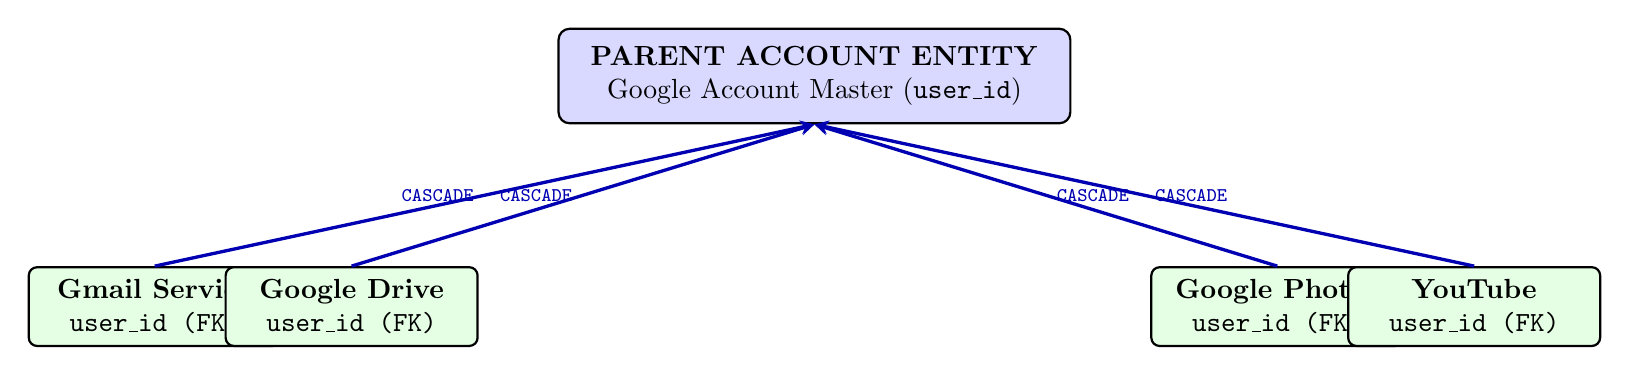
\begin{tikzpicture}[
    node distance=1.5cm and 1.2cm,
    parentbox/.style={draw, rectangle, rounded corners=4pt, thick, fill=blue!15, align=center, minimum width=6.5cm, minimum height=1.2cm},
    childbox/.style={draw, rectangle, rounded corners=3pt, thick, fill=green!10, align=center, minimum width=3.2cm, minimum height=1.0cm},
    arrow/.style={->, >=stealth, very thick, color=blue!70!black}
]
    % Central Parent
    \node[parentbox] (parent) {\textbf{PARENT ACCOUNT ENTITY}\\Google Account Master (\texttt{user\_id})};
    
    % Downstream Services
    \node[childbox, below left=1.8cm and 3.5cm of parent] (gmail) {\textbf{Gmail Service}\\\texttt{user\_id (FK)}};
    \node[childbox, below left=1.8cm and 1.0cm of parent] (drive) {\textbf{Google Drive}\\\texttt{user\_id (FK)}};
    \node[childbox, below right=1.8cm and 1.0cm of parent] (photos) {\textbf{Google Photos}\\\texttt{user\_id (FK)}};
    \node[childbox, below right=1.8cm and 3.5cm of parent] (yt) {\textbf{YouTube}\\\texttt{user\_id (FK)}};
    
    % Dependency Arrows
    \draw[arrow] (gmail.north) -- node[midway, left, font=\scriptsize] {\texttt{CASCADE}} (parent.south);
    \draw[arrow] (drive.north) -- node[midway, left, font=\scriptsize] {\texttt{CASCADE}} (parent.south);
    \draw[arrow] (photos.north) -- node[midway, right, font=\scriptsize] {\texttt{CASCADE}} (parent.south);
    \draw[arrow] (yt.north) -- node[midway, right, font=\scriptsize] {\texttt{CASCADE}} (parent.south);
\end{tikzpicture}
\caption{The Unified Identity lifecycle architecture. A deletion of the central Google Account cascades across all downstream services, guaranteeing complete personal data purging in compliance with data privacy mandates.}
\label{fig:google_sso}
\end{figure*}

\subsubsection{Architectural Policy Analysis}
In this unified identity architecture, the appropriate referential policies are:
\begin{itemize}
    \item \texttt{ON UPDATE CASCADE}: If the account's internal routing identifier changes, that change is immediately synchronized across Drive, Photos, and Gmail tables.
    \item \texttt{ON DELETE CASCADE}: When a user requests permanent account termination under data privacy legislation (e.g., GDPR Right to be Forgotten), the database must guarantee complete eradication of all associated files, mailboxes, and photos. Leaving orphan records in Drive or Photos after the central account is deleted would represent a major regulatory violation and security flaw.
\end{itemize}

\subsection{Case Study B: E-Commerce Audit Trails and Settlement (The Amazon Order Model)}
Now contrast the identity lifecycle with an e-commerce order processing platform such as Amazon:
\begin{itemize}
    \item \textbf{Parent Entities}: 
    \begin{enumerate}
        \item \texttt{customers} (\texttt{customer\_id}, \texttt{name}, \texttt{shipping\_address})
        \item \texttt{saved\_payment\_methods} (\texttt{card\_id}, \texttt{customer\_id}, \texttt{tokenized\_card\_number})
    \end{enumerate}
    \item \textbf{Child Entities}: 
    \begin{enumerate}
        \item \texttt{orders} (\texttt{order\_id}, \texttt{customer\_id}, \texttt{payment\_card\_id}, \texttt{total\_amount}, \texttt{tax\_paid})
        \item \texttt{order\_items} (\texttt{item\_id}, \texttt{order\_id}, \texttt{sku}, \texttt{price})
    \end{enumerate}
\end{itemize}

\subsubsection{Architectural Policy Analysis}
What occurs when a customer deletes an expired credit card from their profile, or even closes their retail purchasing account?
\begin{itemize}
    \item \textbf{Catastrophic Failure of CASCADE}: If \texttt{orders} had an \texttt{ON DELETE CASCADE} relationship with \texttt{saved\_payment\_methods}, deleting an expired Visa card would trigger the database engine to \textbf{delete all historical orders} ever placed with that card! This would destroy taxable transaction logs, eliminate fulfillment records, and wipe out company revenue history.
    \item \textbf{The SET NULL / Immutability Architecture}: To ensure financial compliance, historical orders must never be deleted. 
    The foreign key on \texttt{payment\_card\_id} is configured with \texttt{ON DELETE SET NULL}. If the customer deletes their saved credit card, the historical order retains all fulfillment data, while the payment reference safely transitions to null (with financial audit tokens preserved in an immutable transaction ledger).
    Furthermore, customer account deactivations use Soft Deletion flags (\texttt{is\_active = false}) rather than physical deletions, preserving complete referential integrity across fiscal audit cycles.
\end{itemize}

% -----------------------------------------------------------------------------
\section{Production SQL Implementation Protocols}
\label{sec:sql_implementation}

This section provides complete, syntactically validated SQL scripts demonstrating database lifecycle management, strict referential constraint definitions, and transactional validation using the Academy domain model analyzed in Section~\ref{sec:referential_integrity}.

\subsection{Database Creation and Context Selection}
Every schema definition begins by provisioning an isolated database namespace and establishing execution context:

\begin{lstlisting}[language=SQL]
-- 1. Create the dedicated database namespace
CREATE DATABASE IF NOT EXISTS academy_db
  CHARACTER SET utf8mb4
  COLLATE utf8mb4_unicode_ci;

-- 2. Switch session context to the new database
USE academy_db;
\end{lstlisting}

\subsection{Parent Table Definition: batches}
The parent table must be provisioned first. It establishes the primary key anchor:

\begin{lstlisting}[language=SQL]
-- Create the parent table
CREATE TABLE IF NOT EXISTS batches (
    b_id INT AUTO_INCREMENT PRIMARY KEY,
    batch_name VARCHAR(100) NOT NULL,
    instructor_name VARCHAR(100) NOT NULL,
    created_at TIMESTAMP DEFAULT CURRENT_TIMESTAMP
) ENGINE=InnoDB;
\end{lstlisting}

\subsection{Child Table Definition with Referential Actions: students}
The child table defines the foreign key constraint, enforcing both \texttt{ON UPDATE CASCADE} and \texttt{ON DELETE SET NULL}:

\begin{lstlisting}[language=SQL]
-- Create the child table referencing batches
CREATE TABLE IF NOT EXISTS students (
    s_id INT AUTO_INCREMENT PRIMARY KEY,
    student_name VARCHAR(100) NOT NULL,
    email VARCHAR(150) NOT NULL UNIQUE,
    psp DOUBLE NOT NULL,
    batch_id INT NULL,
    created_at TIMESTAMP DEFAULT CURRENT_TIMESTAMP,
    
    -- Explicit Foreign Key Constraint
    CONSTRAINT fk_students_batches
        FOREIGN KEY (batch_id) 
        REFERENCES batches(b_id)
        ON UPDATE CASCADE
        ON DELETE SET NULL
) ENGINE=InnoDB;
\end{lstlisting}

\subsection{Data Manipulation: Populating Master and Dependent Data}
Data insertion must adhere to dependency order: parent records first, followed by child records referencing valid parent identifiers:

\begin{lstlisting}[language=SQL]
-- 1. Seed Parent Batches
INSERT INTO batches (b_id, batch_name, instructor_name) 
VALUES
    (10, 'SQL & Relational Databases', 'Rohit'),
    (20, 'Low-Level Design Masterclass', 'Umang'),
    (30, 'High-Level System Design', 'Aman');

-- 2. Seed Dependent Student Tuples
INSERT INTO students (s_id, student_name, email, psp, batch_id) 
VALUES
    (1, 'John Doe', 'john@academy.edu', 80.0, 10),
    (2, 'Jane Brown', 'jane@academy.edu', 85.0, 30),
    (3, 'Jim Smith', 'jim@academy.edu', 83.0, 10),
    (4, 'Jack Johnson', 'jack@academy.edu', 99.0, 20),
    (5, 'Jenny Doe', 'jenny@academy.edu', 92.5, 20);
\end{lstlisting}

\subsection{Data Retrieval and Relational Projections}
Standard queries project attributes across the referential boundary using structured joins and conditional filters:

\begin{lstlisting}[language=SQL]
-- Project students with their corresponding batch details
SELECT 
    s.s_id,
    s.student_name,
    s.psp,
    b.batch_name,
    b.instructor_name
FROM students s
LEFT JOIN batches b ON s.batch_id = b.b_id
ORDER BY s.s_id ASC;
\end{lstlisting}

\subsection{Verification of Constraint Enforcement}

\subsubsection{Test 1: Child Insertion with Invalid Foreign Key}
Attempting to insert a student pointing to non-existent batch 99:
\begin{lstlisting}[language=SQL]
-- This statement will fail with MySQL Error 1452
INSERT INTO students (student_name, email, psp, batch_id) 
VALUES ('Orphan Candidate', 'orphan@academy.edu', 75.0, 99);
\end{lstlisting}
The engine halts execution:
\begin{verbatim}
ERROR 1452 (23000): Cannot add or update a child row:
a foreign key constraint fails (`academy_db`.`students`,
CONSTRAINT `fk_students_batches` FOREIGN KEY (`batch_id`)
REFERENCES `batches` (`b_id`) ON UPDATE CASCADE ON DELETE SET NULL)
\end{verbatim}

\subsubsection{Test 2: Verification of ON UPDATE CASCADE}
Updating batch 10 to identifier 15 in the parent table:
\begin{lstlisting}[language=SQL]
UPDATE batches SET b_id = 15 WHERE b_id = 10;
\end{lstlisting}
Querying the child table reveals that students 1 and 3 (previously associated with batch 10) have automatically had their \texttt{batch\_id} updated to 15 without issuing an explicit update against \texttt{students}:
\begin{verbatim}
+------+------------+------+----------+
| s_id | name       | psp  | batch_id |
+------+------------+------+----------+
|    1 | John Doe   | 80.0 |       15 |
|    3 | Jim Smith  | 83.0 |       15 |
+------+------------+------+----------+
\end{verbatim}

\subsubsection{Test 3: Verification of ON DELETE SET NULL}
Deleting batch 20 from the parent table:
\begin{lstlisting}[language=SQL]
DELETE FROM batches WHERE b_id = 20;
\end{lstlisting}
Querying students 4 and 5 (formerly in batch 20) reveals that their records remain intact, but their \texttt{batch\_id} attribute has transitioned cleanly to \texttt{NULL}:
\begin{verbatim}
+------+--------------+------+----------+
| s_id | name         | psp  | batch_id |
+------+--------------+------+----------+
|    4 | Jack Johnson | 99.0 |     NULL |
|    5 | Jenny Doe    | 92.5 |     NULL |
+------+--------------+------+----------+
\end{verbatim}
Referential integrity is maintained, no orphan records exist, and zero application data was lost.

% -----------------------------------------------------------------------------
\section{The Sakila Reference Database Architecture}
\label{sec:sakila_architecture}

To observe relational integrity across industrial-scale schemas, database engineers frequently reference the canonical \textbf{Sakila} database. Sakila was designed by MySQL architects to model a commercial video rental enterprise, incorporating complex referential constraints, composite keys, and cascade chains.

\subsection{Core Entity Relationships in Sakila}
Sakila demonstrates multi-tiered foreign key dependencies across four functional operational domains:
\begin{enumerate}
    \item \textbf{Inventory and Catalog Management}:
    \begin{itemize}
        \item \texttt{film} relates to \texttt{language} via foreign key \texttt{language\_id}.
        \item \texttt{film\_actor} acts as a many-to-many junction table between \texttt{film} and \texttt{actor}, utilizing a Composite Primary Key consisting of \texttt{(actor\_id, film\_id)}.
        \item \texttt{inventory} represents physical stock copies in stores, holding foreign keys referencing both \texttt{film(film\_id)} and \texttt{store(store\_id)}.
    \end{itemize}
    \item \textbf{Customer Operations and Rentals}:
    \begin{itemize}
        \item \texttt{rental} captures the temporal checkout event, maintaining foreign keys pointing to \texttt{inventory(inventory\_id)}, \texttt{customer(customer\_id)}, and \texttt{staff(staff\_id)}.
    \end{itemize}
    \item \textbf{Payment Settlement}:
    \begin{itemize}
        \item \texttt{payment} references \texttt{rental(rental\_id)} and \texttt{customer(customer\_id)}, ensuring that financial ledger rows cannot exist without an authorized customer and rental record.
    \end{itemize}
\end{enumerate}

\begin{figure*}[htbp]
\centering
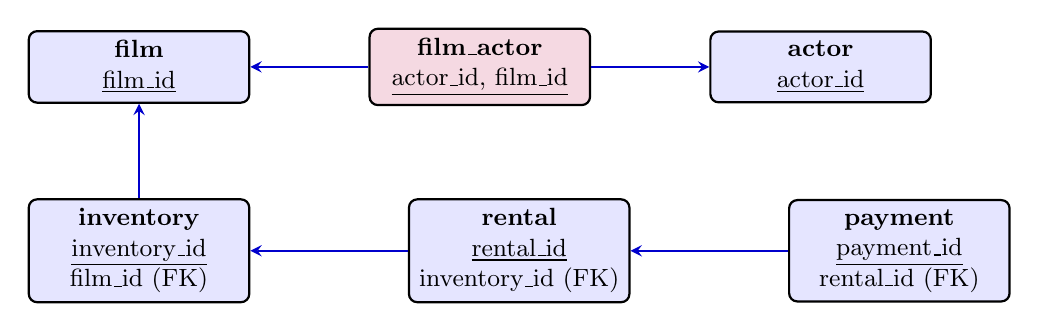
\begin{tikzpicture}[
    node distance=1.0cm and 1.5cm,
    ent/.style={draw, rectangle, rounded corners=3pt, thick, fill=blue!10, align=center, minimum width=2.8cm, minimum height=0.9cm, font=\small},
    junc/.style={draw, rectangle, rounded corners=3pt, thick, fill=purple!15, align=center, minimum width=2.8cm, minimum height=0.9cm, font=\small},
    rel/.style={->, >=stealth, thick, color=blue!80!black}
]
    \node[ent] (film) {\textbf{film}\\\underline{film\_id}};
    \node[junc, right=of film] (film_actor) {\textbf{film\_actor}\\\underline{actor\_id, film\_id}};
    \node[ent, right=of film_actor] (actor) {\textbf{actor}\\\underline{actor\_id}};
    
    \node[ent, below=1.2cm of film] (inventory) {\textbf{inventory}\\\underline{inventory\_id}\\film\_id (FK)};
    \node[ent, right=2.0cm of inventory] (rental) {\textbf{rental}\\\underline{rental\_id}\\inventory\_id (FK)};
    \node[ent, right=2.0cm of rental] (payment) {\textbf{payment}\\\underline{payment\_id}\\rental\_id (FK)};
    
    \draw[rel] (film_actor) -- (film);
    \draw[rel] (film_actor) -- (actor);
    \draw[rel] (inventory) -- (film);
    \draw[rel] (rental) -- (inventory);
    \draw[rel] (payment) -- (rental);
\end{tikzpicture}
\caption{Architectural dependency graph of the canonical Sakila database. Foreign key linkages bind inventory, rentals, and payments, preventing orphaned transactions across multi-tiered relational workflows.}
\label{fig:sakila_graph}
\end{figure*}

\subsection{Architectural Lessons from Sakila}
The Sakila schema highlights two critical production guidelines:
\begin{itemize}
    \item \textbf{Every Foreign Key Must Be Indexed}: In the child table \texttt{rental}, the column \texttt{inventory\_id} is a foreign key. MySQL automatically creates an index on this foreign key column. Without this index, any deletion or update in the parent \texttt{inventory} table would force the database engine to perform a full table scan across millions of \texttt{rental} rows to verify referential integrity, resulting in severe lock contention.
    \item \textbf{Strict Isolation of Financials}: Payments in Sakila reference rentals, but historical payments are protected from cascade deletion via \texttt{RESTRICT} rules, preventing accidental loss of financial accounting records.
\end{itemize}

% -----------------------------------------------------------------------------
\section{Production Engineering Best Practices}
\label{sec:best_practices}

To conclude this architectural analysis, we outline essential engineering guidelines for database designers building high-throughput relational systems:

\begin{enumerate}
    \item \textbf{Always Use Compact Surrogate Primary Keys}: Standardize on 4-byte \texttt{INT} or 8-byte \texttt{BIGINT} auto-incrementing identifiers for primary keys. Never use national identification numbers, phone numbers, or unhashed email strings as primary keys.
    \item \textbf{Index Every Foreign Key Column}: Database engines automatically create indexes on Primary Keys, but they do not always automatically index Foreign Key columns in child tables. Always verify that an index exists on every foreign key column to prevent full table scans and row locks during parent table mutations.
    \item \textbf{Explicitly Declare Referential Rules}: Never leave foreign key actions to implicit defaults. Always explicitly define \texttt{ON UPDATE CASCADE} and either \texttt{ON DELETE RESTRICT} or \texttt{ON DELETE SET NULL} to make business intent unmistakable in schema DDL.
    \item \textbf{Avoid Deep Cascade Trees}: Chaining \texttt{CASCADE} rules across five or six hierarchical tiers (e.g., Company to Department to Team to Project to Task to Comment) creates massive transactional lock cascades. A single deletion at the root can lock hundreds of thousands of rows, leading to transaction timeouts and deadlocks. In deeply nested architectures, utilize asynchronous soft deletion workers instead of synchronous deep database cascades.
    \item \textbf{Enforce Alternate Key Uniqueness Independently}: Protect natural keys (such as email and phone numbers) using explicit \texttt{UNIQUE} constraints rather than overloading them as primary keys.
\end{enumerate}

% -----------------------------------------------------------------------------
\section{Conclusion}
\label{sec:conclusion}

Relational database integrity is the bedrock of dependable software engineering. By understanding the physical reality of primary key clustered indexes, the storage footprint overhead of candidate keys, and the operational mechanics of foreign key referential constraints, software engineers can design resilient, high-throughput architectures that completely eliminate orphan records and update anomalies. 

This paper has demonstrated the complete taxonomy of relational keys, proved why compact immutable surrogate integers outperform natural strings as primary keys, detailed the exact operational mechanics of \texttt{ON UPDATE} and \texttt{ON DELETE} rules (\texttt{CASCADE}, \texttt{SET NULL}, \texttt{RESTRICT}), analyzed production case studies from Google SSO and Amazon Order management, and provided validated SQL implementation protocols. Adherence to these engineering principles ensures that relational systems remain both performant under massive scale and structurally immutable against data corruption.

% -----------------------------------------------------------------------------
\begin{thebibliography}{10}

\bibitem{codd1970}
E.~F.~Codd, ``A Relational Model of Data for Large Shared Data Banks,'' \emph{Communications of the ACM}, vol.~13, no.~6, pp.~377--387, 1970.

\bibitem{date2004}
C.~J.~Date, \emph{An Introduction to Database Systems}, 8th~ed.\hskip 1em plus 0.5em minus 0.4em\relax Boston: Addison-Wesley, 2004.

\bibitem{silberschatz2020}
A.~Silberschatz, H.~F.~Korth, and S.~Sudarshan, \emph{Database System Concepts}, 7th~ed.\hskip 1em plus 0.5em minus 0.4em\relax New York: McGraw-Hill, 2020.

\bibitem{mysql2024}
Oracle Corporation, ``MySQL 8.4 Reference Manual: InnoDB Storage Engine and Clustered Indexes,'' Oracle Technology Network, 2024. [Online]. Available: \url{https://dev.mysql.com/doc/refman/8.4/en/innodb-index-types.html}

\bibitem{sakila2024}
Oracle Corporation, ``Sakila Sample Database Architecture and Schema Documentation,'' Oracle Corporation, 2024. [Online]. Available: \url{https://dev.mysql.com/doc/sakila/en/}

\end{thebibliography}


\end{document}
